\documentclass[12pt, letterpaper]{article}
\usepackage[utf8]{inputenc}
\usepackage[spanish]{babel}
\usepackage{amsmath}
\usepackage{amssymb}
\usepackage{graphicx}
\usepackage[margin=1in]{geometry}
\usepackage{hyperref}
\usepackage{parskip}


\title{Tarea 1: Computación de Alto Rendimiento (IIC3533)}
\author{Josefina Abbott Cerda, José Ignacio Salas Coeymans y Borja Smith Vergara}
\date{11 de septiembre de 2026}

\begin{document}

\maketitle

\section*{(a) Generación de datos sintéticos}
Para generar los datos sintéticos, seguimos los siguientes pasos:

\begin{enumerate}
    \item Generar los datos, usando el generador aleatorio de NumPy (\texttt{np.random.default\_rng}) fijando una semilla base, nosotros la establecimos como 1111.
    \item Generar el vector de coeficientes reales $\beta^* \in \mathbb{R}^{301}$ muestreando de una distribución normal estándar $\mathcal{N}(0,1)$. 
    \item Crear una matriz base de $10000 \times 300$ con valores independientes $\mathcal{N}(0,1)$.
    \item Concatenar horizontalmente un vector columna de unos a la matriz base para incorporar el intercepto ($\beta_0$), obteniendo así la matriz de diseño $X \in \mathbb{R}^{10000 \times 301}$.
    \item Calcular el vector de respuesta $y \in \mathbb{R}^{10000}$ con el producto matricial $y = X\beta^* + \varepsilon$, donde $\varepsilon$ es un vector de ruido con $10000$ muestras i.i.d. de $\mathcal{N}(0,1)$.
\end{enumerate}

Para correr el script de generación de datos, se puede ejecutar el siguiente comando en la terminal:
\begin{verbatim}
python src/data_generation.py
\end{verbatim}

\section*{(b) Implementaciones de bootstrapping}

\subsection*{Evolución de \texttt{bs\_auto.py}}

\textbf{1. Cambios implementados por versión}
\begin{itemize}
    \item \textbf{Versión 1 (Ingenua):} Utiliza la configuración por defecto de scikit-learn. Emplea \texttt{LinearRegression()} pese a que $X$ ya contiene una columna de unos; además, al guardar solamente \texttt{coef\_}, pierde el intercepto separado del modelo. Por ello esta versión sirve como punto de partida, pero no entrega correctamente el intervalo de $\beta_0$.
    \item \textbf{Versión 2:} Introduce \texttt{fit\_intercept=False}. Dado que la matriz de diseño $X$ ya incluye una columna de unos pre-concatenada, esto evita el cálculo de un intercepto redundante.
    \item \textbf{Versión 3:} Reemplaza el ciclo \texttt{for} por una comprensión de listas para expresar de forma más compacta la extracción de coeficientes. Este cambio no vectoriza los ajustes ni garantiza por sí solo una mejora medible.
    \item \textbf{Versión 4:} Declara explícitamente \texttt{bootstrap=True} (aunque ya es el valor por defecto) y fija \texttt{random\_state=1234}, garantizando muestreo con reemplazo y reproducibilidad.
    \item \textbf{Versión 5:} Mantiene los parámetros óptimos del modelo, pero revierte la extracción de coeficientes al ciclo \texttt{for} con \texttt{.append()} para contrastar el manejo de memoria final.
\end{itemize}

\textbf{2. Tiempos de ejecución}

\begin{table}[h]
    \centering
    \begin{tabular}{|c|l|c|}
    \hline
    \textbf{Versión} & \textbf{Características Principales} & \textbf{Tiempo ($p=1$)} \\
    \hline
    v1 & Intercepto activo, ciclo for & 4.7474 s \\
    v2 & Sin intercepto, ciclo for & 5.1836 s \\
    v3 & Sin intercepto, list comprehension & 5.3599 s \\
    v4 & Sin inter., list comp., bootstrap explícito & 4.2048 s \\
    v5 & Sin inter., ciclo for, bootstrap explícito & 4.1570 s \\
    \hline
    \end{tabular}
    \caption{Tiempos de ejecución empíricos para distintas iteraciones de \texttt{bs\_auto.py}.}
\end{table}

\textbf{3. Análisis de la versión óptima}

La \textbf{Versión 4} es computacional y estructuralmente la más óptima. 

En primer lugar, al definir \texttt{fit\_intercept=False}, se evita estimar un intercepto separado cuando la matriz $X$ ya incluye la columna de unos. Declarar \texttt{bootstrap=True} hace explícito el remuestreo exigido, mientras que \texttt{random\_state} permite reproducir los mismos intervalos al cambiar el número de procesos.

Si bien la Versión 5 registró un tiempo marginalmente inferior en esa
ejecución (4.15 s frente a 4.20 s), una diferencia de 0.05 s no permite afirmar
que una forma de extraer 48 vectores sea más rápida. Elegimos la Versión 4 por
claridad, concisión y reproducibilidad, no por esa diferencia aislada.

\subsection*{Evolución de \texttt{bs\_sklearn.py}}

\textbf{1. Cambios implementados por versión}
\begin{itemize}
    \item \textbf{Versión 1 (Ingenua):} Utiliza el generador aleatorio global (\texttt{np.random.choice}) dentro de cada proceso trabajador. Su estado no queda asignado explícitamente a cada remuestreo y, dependiendo de cómo se creen los procesos, puede producir secuencias duplicadas o resultados no reproducibles. Además, mantiene activado el cálculo del intercepto por defecto.
    \item \textbf{Versión 2:} Aísla la generación de números aleatorios asignando una semilla determinista única (\texttt{seed\_b}) a cada proceso mediante \texttt{np.random.default\_rng(seed\_b)}. Esto incrementa levemente el tiempo de ejecución por el costo de instanciar 48 generadores distintos, pero es matemáticamente obligatorio para garantizar la validez estadística.
    \item \textbf{Versión 3:} Introduce \texttt{fit\_intercept=False}. Al igual que en \texttt{bs\_auto.py}, esto elimina el procesamiento redundante de la matriz, reduciendo los tiempos de ejecución sin cambiar el vector de coeficientes retornado a los procesos trabajadores.
\end{itemize}

\textbf{2. Tiempos de ejecución}

\begin{table}[h]
    \centering
    \begin{tabular}{|c|l|c|}
    \hline
    \textbf{Versión} & \textbf{Características Principales} & \textbf{Tiempo ($p=1$)} \\
    \hline
    v1 & RNG global (incorrecto), intercepto activo & 5.9958 s \\
    v2 & RNG independiente (correcto), intercepto activo & 7.7394 s \\
    v3 & RNG independiente, sin intercepto & 5.5406 s \\
    \hline
    \end{tabular}
    \caption{Tiempos de ejecución empíricos para distintas iteraciones de \texttt{bs\_sklearn.py}.}
\end{table}

\textbf{3. Análisis de la versión óptima}

La \textbf{Versión 3} representa la implementación correcta y más eficiente utilizando scikit-learn de forma explícita. El manejo independiente de las semillas elimina las condiciones de carrera paralela, mientras que la desactivación del intercepto evita cálculos innecesarios sobre la matriz $X$, devolviendo el tiempo de ejecución a niveles óptimos ($\sim$5.54s) sin comprometer la correctitud del algoritmo iterativo.

\subsection*{Evolución de \texttt{bs\_numpy.py}}

\textbf{1. Cambios implementados por versión}
\begin{itemize}
    \item \textbf{Versión 1 (Ingenua):} Traduce literalmente la fórmula de Mínimos Cuadrados Ordinarios entregada en el enunciado: $\hat{\beta} = (X^{\top}X)^{-1}X^{\top}y$. Utiliza \texttt{np.linalg.inv()} para calcular explícitamente la matriz inversa antes de realizar las multiplicaciones matriciales.
    \item \textbf{Versión 2:} Reemplaza la inversión explícita reescribiendo el problema como la resolución de un sistema de ecuaciones lineales: $(X^{\top}X)\hat{\beta} = X^{\top}y$. Utiliza \texttt{np.linalg.solve()} para encontrar los coeficientes de manera directa.
\end{itemize}

\textbf{2. Tiempos de ejecución}

\begin{table}[h]
    \centering
    \begin{tabular}{|c|l|c|}
    \hline
    \textbf{Versión} & \textbf{Características Principales} & \textbf{Tiempo ($p=1$)} \\
    \hline
    v1 & Cálculo explícito con \texttt{np.linalg.inv()} & 1.0937 s \\
    v2 & Resolución de sistema con \texttt{np.linalg.solve()} & 1.0204 s \\
    \hline
    \end{tabular}
    \caption{Tiempos de ejecución empíricos para distintas iteraciones de \texttt{bs\_numpy.py}.}
\end{table}

\textbf{3. Análisis de la versión óptima}

La \textbf{Versión 2} es la implementación óptima y definitiva para esta sección. 

Aunque la diferencia de tiempo empírica en una sola ejecución con $p=1$ parece marginal ($\sim$0.07 segundos), el cambio posee un peso teórico y arquitectónico fundamental. Calcular explícitamente la inversa de una matriz mediante \texttt{np.linalg.inv()} es computacionalmente ineficiente y altamente susceptible a errores de redondeo de punto flotante a medida que la dimensionalidad aumenta. 

Al utilizar \texttt{np.linalg.solve()}, NumPy delega la operación a subrutinas optimizadas de álgebra lineal (LAPACK), que resuelven el sistema $(X^{\top}X)\hat{\beta}=X^{\top}y$ sin construir explícitamente la inversa. Esto reduce operaciones y error numérico respecto de \texttt{inv}; no obstante, ambas versiones forman las ecuaciones normales y, por tanto, siguen siendo menos estables que resolver directamente el problema de mínimos cuadrados mediante QR o SVD.

Para correr las implementaciones, se pueden ejecutar los siguientes comandos en la terminal:
\begin{verbatim}
python src/bs_auto.py
python src/bs_sklearn.py
python src/bs_numpy.py
\end{verbatim}

\section*{(c) Correctitud y reproducibilidad}

Primero calculamos $\hat\beta$ sobre el conjunto completo, como indica el paso
1 del algoritmo. El error relativo
$\lVert\hat\beta-\beta^*\rVert_2/\lVert\beta^*\rVert_2$ fue 0.00989, lo que
confirma que el ajuste recupera adecuadamente los coeficientes verdaderos.

Luego ejecutamos cada versión dos veces con $p=1$ y una vez con $p=4$, usando
las mismas semillas. La Tabla~\ref{tab:correctitud-c} resume la cobertura, el
ancho medio de los intervalos y la máxima diferencia entre ejecuciones.

\begin{table}[h]
    \centering
    \small
    \begin{tabular}{|l|r|r|r|r|}
    \hline
    \textbf{Implementación} & \textbf{Cobertura} & \textbf{Ancho medio}
    & \textbf{Rep. $p=1$} & \textbf{$p=1$ vs. $p=4$} \\
    \hline
    BaggingRegressor & 91.36\% & 0.035989 & 0 & 0 \\
    sklearn + joblib & 91.69\% & 0.036064 & 0 & 0 \\
    NumPy + joblib & 91.69\% & 0.036064 & 0 & 0 \\
    \hline
    \end{tabular}
    \caption{Correctitud y reproducibilidad. Las dos últimas columnas muestran
    la máxima diferencia absoluta entre extremos de los intervalos.}
    \label{tab:correctitud-c}
\end{table}

Las coberturas son similares y razonablemente cercanas al 95\% nominal,
considerando que solo se usan $B=48$ remuestreos. Las versiones manuales
emplean exactamente los mismos índices y sus intervalos difieren como máximo
en $2.27\times10^{-14}$, debido al redondeo de las rutinas de álgebra lineal.
\texttt{BaggingRegressor} usa otra secuencia de remuestreo y por eso no produce
los mismos extremos, pero su cobertura y ancho son comparables.

La reproducibilidad requiere fijar la semilla de los datos, asignar una semilla
determinista a cada remuestreo y fijar \texttt{random\_state} en
\texttt{BaggingRegressor}. Como la semilla depende de $b$ y no del worker que
ejecuta la tarea, cambiar $p$ no cambia los intervalos. Los resultados completos
se almacenan en \texttt{results/computer\_1/correctness\_c.csv}.

Para verificar la correctitud y reproducibilidad de las implementaciones, se puede ejecutar el siguiente comando en la terminal:
\begin{verbatim}
python src/correctness.py
\end{verbatim}

\section*{(d) Backend multiprocessing de joblib}

\textbf{Creación de procesos y asignación de memoria:}
\texttt{Parallel} utiliza por defecto el backend basado en procesos
\texttt{loky}. Este crea intérpretes Python separados, cada uno con su propio
espacio de direcciones; por tanto, no debe asumirse que todos los objetos se
comparten automáticamente mediante \textit{fork}. En sistemas que crean procesos
con \textit{fork} puede existir inicialmente \textit{Copy-on-Write}, pero
\texttt{loky} también serializa argumentos para enviarlos a los workers y su
comportamiento depende del sistema operativo.

\textbf{Comportamiento de los arreglos $X$ e $y$:}
Como $X$ supera el umbral de tamaño por defecto de joblib, \texttt{loky} puede
volcarlo automáticamente a un archivo temporal y abrirlo como \textit{memmap} de
solo lectura en los workers. Esto evita serializar una copia completa de $X$ por
tarea. El arreglo $y$ es menor y puede serializarse normalmente. Sin embargo,
la indexación avanzada \texttt{X[indices]} y \texttt{y[indices]} sí crea
arreglos nuevos $X^{(b)}$ e $y^{(b)}$ dentro de cada tarea. Por tanto, se
comparte o mapea la entrada original, pero cada worker necesita memoria
adicional para sus remuestreos y matrices intermedias.

\section*{(e) Actividad del sistema y oversubscription}

Los experimentos de este inciso se realizaron en un MacBook Air con Apple M1,
8 cores (4 de rendimiento y 4 de eficiencia), 8 GB de RAM y macOS
(arquitectura ARM64). Se utilizó NumPy 2.0.2, joblib 1.5.3 y
threadpoolctl 3.6.0. La configuración de NumPy indica que las operaciones BLAS y
LAPACK están enlazadas con el framework Apple Accelerate.

Ejecutamos \texttt{bs\_numpy.py} tres veces con
$p\in\{1,2,4,8\}$. Se observaron exactamente 1, 2, 4 y 8 procesos trabajadores,
respectivamente. En una ejecución prolongada con $p=8$, los workers registraron
aproximadamente entre 53\% y 66\% de CPU cada uno, confirmando que los
remuestreos se distribuyen entre procesos independientes.

\begin{table}[h]
    \centering
    \begin{tabular}{|c|c|c|}
    \hline
    $p$ & \textbf{Workers observados} & \textbf{Tiempo mediano [s]} \\
    \hline
    1 & 1 & 0.536 \\
    2 & 2 & 0.559 \\
    4 & 4 & 0.481 \\
    8 & 8 & 0.470 \\
    \hline
    \end{tabular}
    \caption{Actividad observada al ejecutar la versión NumPy.}
\end{table}

Ejecutamos \texttt{threadpool\_info()} dentro de cada worker, después de cargar
NumPy. En todos los casos retornó una lista vacía. Esta observación es coherente
con que el NumPy instalado usa Apple Accelerate, cuyo pool interno no es
reportado por \texttt{threadpoolctl}. Al cargar SciPy y scikit-learn sí aparecen
un pool OpenBLAS y uno OpenMP de 8 threads, pero estos pertenecen a dichas
bibliotecas y no demuestran que \texttt{np.linalg.solve} use esos pools.

Los tiempos no presentan una degradación al aumentar $p$, por lo que no hay
evidencia directa de \textit{oversubscription} en esta ejecución. No obstante,
la falta de visibilidad sobre Accelerate impide conocer el valor efectivo de
$t$; por ello la conclusión es limitada y no equivale a demostrar que $t=1$.

En general, sí existiría oversubscription si cada uno de los $p$ procesos
lanzara $t$ threads BLAS y se cumpliera $p\,t>p_{\max}$. En una instalación
compatible con \texttt{threadpoolctl} puede corregirse envolviendo el cálculo
de cada worker con \texttt{threadpool\_limits(limits=1)} o configurando
\texttt{inner\_max\_num\_threads=1} en el backend \texttt{loky}. Para Apple
Accelerate puede fijarse \texttt{VECLIB\_MAXIMUM\_THREADS=1} antes de iniciar
Python. Las observaciones completas quedaron almacenadas en
\texttt{results/computer\_1/observations\_e.csv}.

\section*{(f) Tiempos de ejecución en función de p}

El primer computador posee $p_{\max}=8$ cores lógicos. Comparamos las
versiones finales \texttt{bootstrap\_auto\_v4},
\texttt{bootstrap\_sklearn\_v3} y \texttt{bootstrap\_numpy\_v2} usando los
mismos datos ($N=10000$, $k=300$), $B=48$ y las mismas semillas. Para cada
implementación y cada $p\in\{1,\ldots,8\}$ se realizaron cinco ejecuciones,
cada una en un intérprete Python nuevo para impedir que joblib reutilizara un
pool creado por una medición anterior. El orden de las 120 configuraciones fue aleatorizado para reducir el sesgo causado
por calentamiento del equipo o por el orden de ejecución. Reportamos la mediana,
por ser menos sensible que la media a interferencias transitorias del sistema.

\begin{table}[h]
    \centering
    \small
    \begin{tabular}{|c|r|r|r|}
    \hline
    $p$ & \textbf{BaggingRegressor} & \textbf{sklearn + joblib} & \textbf{NumPy + joblib} \\
    \hline
    1 & 13.988 & 10.658 & 0.614 \\
    2 & 7.866 & 8.051 & 0.733 \\
    3 & 5.000 & 5.308 & 0.716 \\
    4 & 4.816 & 5.069 & 0.710 \\
    5 & 4.160 & 4.602 & 0.763 \\
    6 & 4.381 & 4.591 & 0.825 \\
    7 & 4.193 & 4.899 & 0.793 \\
    8 & 4.379 & 4.773 & 0.811 \\
    \hline
    \end{tabular}
    \caption{Mediana de los tiempos de ejecución $T(p)$, en segundos, para
    cinco repeticiones aisladas en el primer computador.}
    \label{tab:tiempos-f}
\end{table}

\begin{figure}[h]
    \centering
    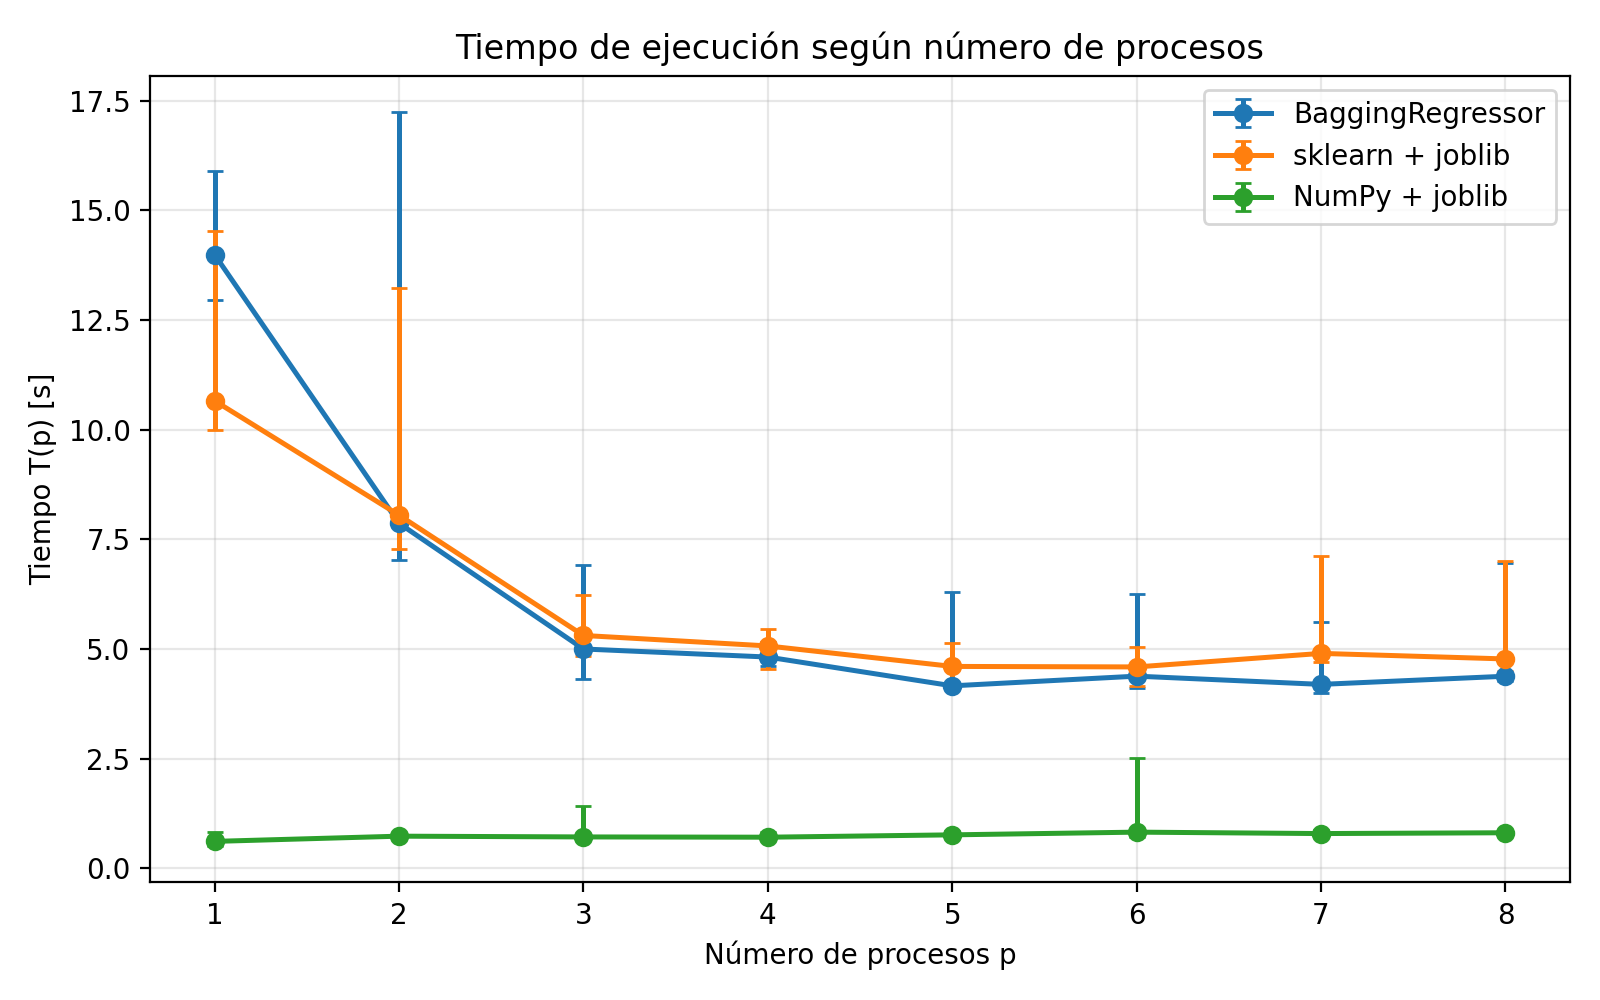
\includegraphics[width=0.82\textwidth]{../results/computer_1/tiempos_f.png}
    \caption{Tiempo mediano de ejecución en función de $p$. Las barras se
    extienden entre el mínimo y el máximo de las cinco repeticiones.}
    \label{fig:tiempos-f}
\end{figure}

La implementación basada solamente en NumPy fue la más rápida para todos los
valores de $p$: con un proceso tardó aproximadamente 0.614 s, frente a 13.988 s
de \texttt{BaggingRegressor} y 10.658 s de la versión manual con scikit-learn.
La diferencia se debe principalmente a que \texttt{LinearRegression} realiza
más trabajo general para ajustar cada modelo, mientras que la versión NumPy
resuelve directamente las ecuaciones normales.

Las dos implementaciones basadas en scikit-learn mejoraron al aumentar $p$
hasta aproximadamente cinco o seis procesos. El mejor tiempo mediano fue
4.160 s con $p=5$ para \texttt{BaggingRegressor} y 4.591 s con $p=6$ para
\texttt{sklearn + joblib}. En cambio, NumPy no escaló al aumentar los procesos:
su menor tiempo fue 0.614 s con $p=1$ y todas las configuraciones paralelas
fueron más lentas. En esta versión cada tarea es
tan breve que el costo de crear o coordinar procesos, despachar las 48 tareas y
administrar sus resultados supera el beneficio. En las versiones de
scikit-learn, usar más de cinco o seis procesos tampoco mejora de forma estable,
debido al overhead y a la competencia por recursos compartidos.

\section*{(g) Speedup S(p) y Eficiencia E(p)}

A partir de las medianas de la Tabla~\ref{tab:tiempos-f}, calculamos para cada
implementación:
\[
    S(p)=\frac{T(1)}{T(p)}, \qquad E(p)=\frac{S(p)}{p}.
\]
Elegimos como $T(1)$ la mediana de las cinco ejecuciones de la misma
implementación con $p=1$: 13.988 s para \texttt{BaggingRegressor}, 10.658 s para
\texttt{sklearn + joblib} y 0.614 s para \texttt{NumPy + joblib}. Esta elección
mantiene constantes el algoritmo, los datos, las semillas y la instrumentación,
por lo que mide escalabilidad fuerte sin mezclar el resultado con una
implementación secuencial diferente. Además, usar la mediana evita que una
ejecución excepcionalmente lenta o rápida determine toda la curva.

\begin{table}[h]
    \centering
    \scriptsize
    \begin{tabular}{|c|cc|cc|cc|}
    \hline
     & \multicolumn{2}{c|}{\textbf{BaggingRegressor}}
     & \multicolumn{2}{c|}{\textbf{sklearn + joblib}}
     & \multicolumn{2}{c|}{\textbf{NumPy + joblib}} \\
    $p$ & $S(p)$ & $E(p)$ & $S(p)$ & $E(p)$ & $S(p)$ & $E(p)$ \\
    \hline
    1 & 1.000 & 1.000 & 1.000 & 1.000 & 1.000 & 1.000 \\
    2 & 1.778 & 0.889 & 1.324 & 0.662 & 0.838 & 0.419 \\
    3 & 2.798 & 0.933 & 2.008 & 0.669 & 0.858 & 0.286 \\
    4 & 2.904 & 0.726 & 2.102 & 0.526 & 0.865 & 0.216 \\
    5 & 3.363 & 0.673 & 2.316 & 0.463 & 0.805 & 0.161 \\
    6 & 3.193 & 0.532 & 2.322 & 0.387 & 0.745 & 0.124 \\
    7 & 3.336 & 0.477 & 2.175 & 0.311 & 0.775 & 0.111 \\
    8 & 3.194 & 0.399 & 2.233 & 0.279 & 0.757 & 0.095 \\
    \hline
    \end{tabular}
    \caption{Speedup y eficiencia calculados a partir de los tiempos medianos.}
    \label{tab:metricas-g}
\end{table}

\begin{figure}[h]
    \centering
    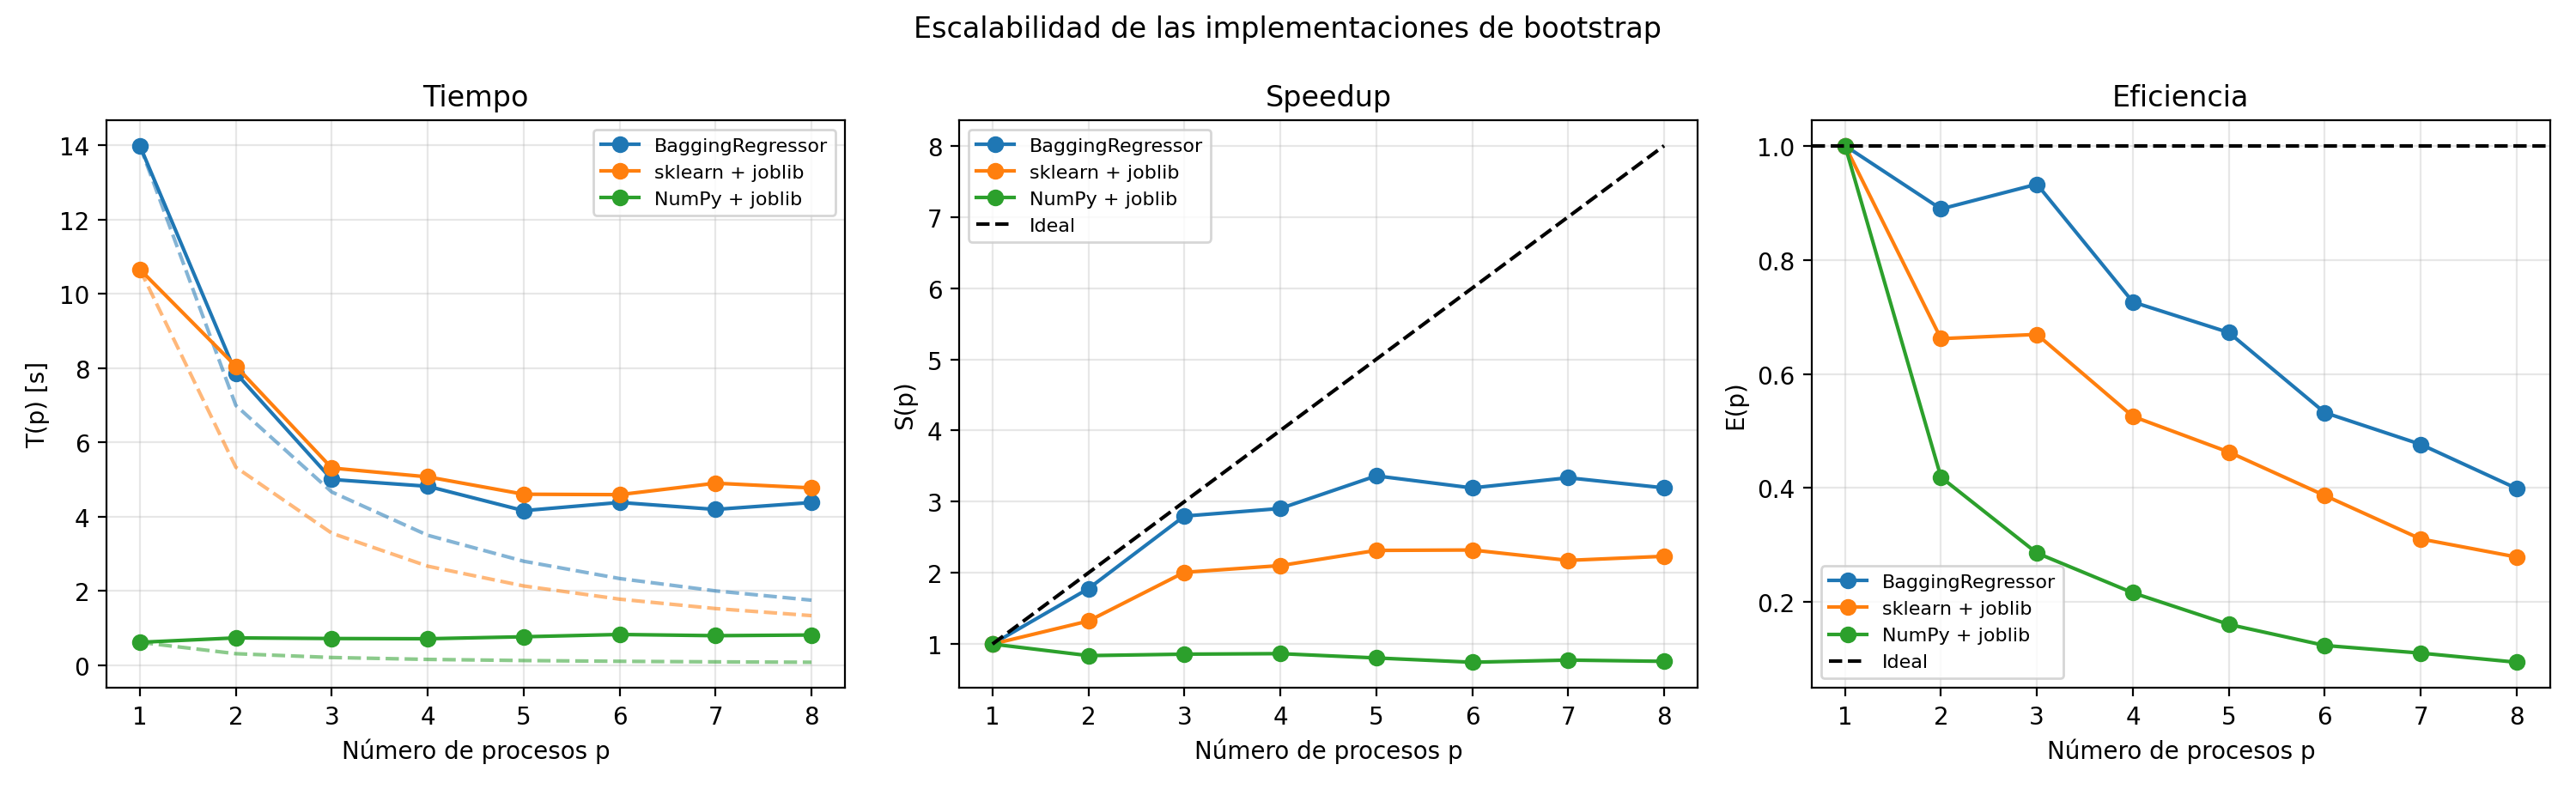
\includegraphics[width=\textwidth]{../results/computer_1/metricas_g.png}
    \caption{Tiempo, speedup y eficiencia observados. En el panel de tiempo,
    las líneas discontinuas corresponden a $T(1)/p$ para cada implementación;
    en los otros paneles, la curva ideal es $S(p)=p$ y $E(p)=1$.}
    \label{fig:metricas-g}
\end{figure}

Ninguna implementación alcanzó la curva ideal. \texttt{BaggingRegressor}
obtuvo su mayor speedup en $p=5$, con $S(5)=3.363$ y $E(5)=0.673$. La versión
manual con scikit-learn alcanzó su máximo en $p=6$, con $S(6)=2.322$ y
$E(6)=0.387$. En ambas versiones el trabajo de ajustar 48 regresiones es
suficiente para amortizar parte del costo de los procesos, pero la eficiencia
disminuye al crecer $p$ debido a creación y coordinación de procesos,
distribución de tareas, movimiento de resultados y competencia por memoria.

La versión NumPy presenta un comportamiento distinto. Su tiempo con un solo
proceso ya es muy bajo, de modo que el overhead paralelo domina: para todos los
valores $p>1$ se obtuvo $S(p)<1$. Su eficiencia cae
desde 0.419 con $p=2$ hasta 0.095 con $p=8$. Por lo tanto, en este computador la
implementación NumPy es la más rápida en tiempo absoluto, pero su configuración
más razonable es $p=1$; paralelizarla no entrega una mejora robusta para
$B=48$, $N=10000$ y $k=300$.

\section*{(h) Overhead $T_o(p)$}

Definimos el overhead total como
\[
    T_o(p)=pT(p)-T(1),
\]
que mide el tiempo-procesador adicional respecto de la ejecución con un solo
proceso. Por definición, $T_o(1)=0$.

\begin{table}[h]
    \centering
    \small
    \begin{tabular}{|c|r|r|r|}
    \hline
    $p$ & \textbf{BaggingRegressor} & \textbf{sklearn + joblib} & \textbf{NumPy + joblib} \\
    \hline
    1 & 0.000 & 0.000 & 0.000 \\
    2 & 1.744 & 5.444 & 0.852 \\
    3 & 1.011 & 5.266 & 1.533 \\
    4 & 5.277 & 9.620 & 2.225 \\
    5 & 6.811 & 12.355 & 3.202 \\
    6 & 12.296 & 16.887 & 4.335 \\
    7 & 15.363 & 23.638 & 4.934 \\
    8 & 21.043 & 27.524 & 5.873 \\
    \hline
    \end{tabular}
    \caption{Overhead total $T_o(p)$, en segundos.}
\end{table}

\begin{figure}[h]
    \centering
    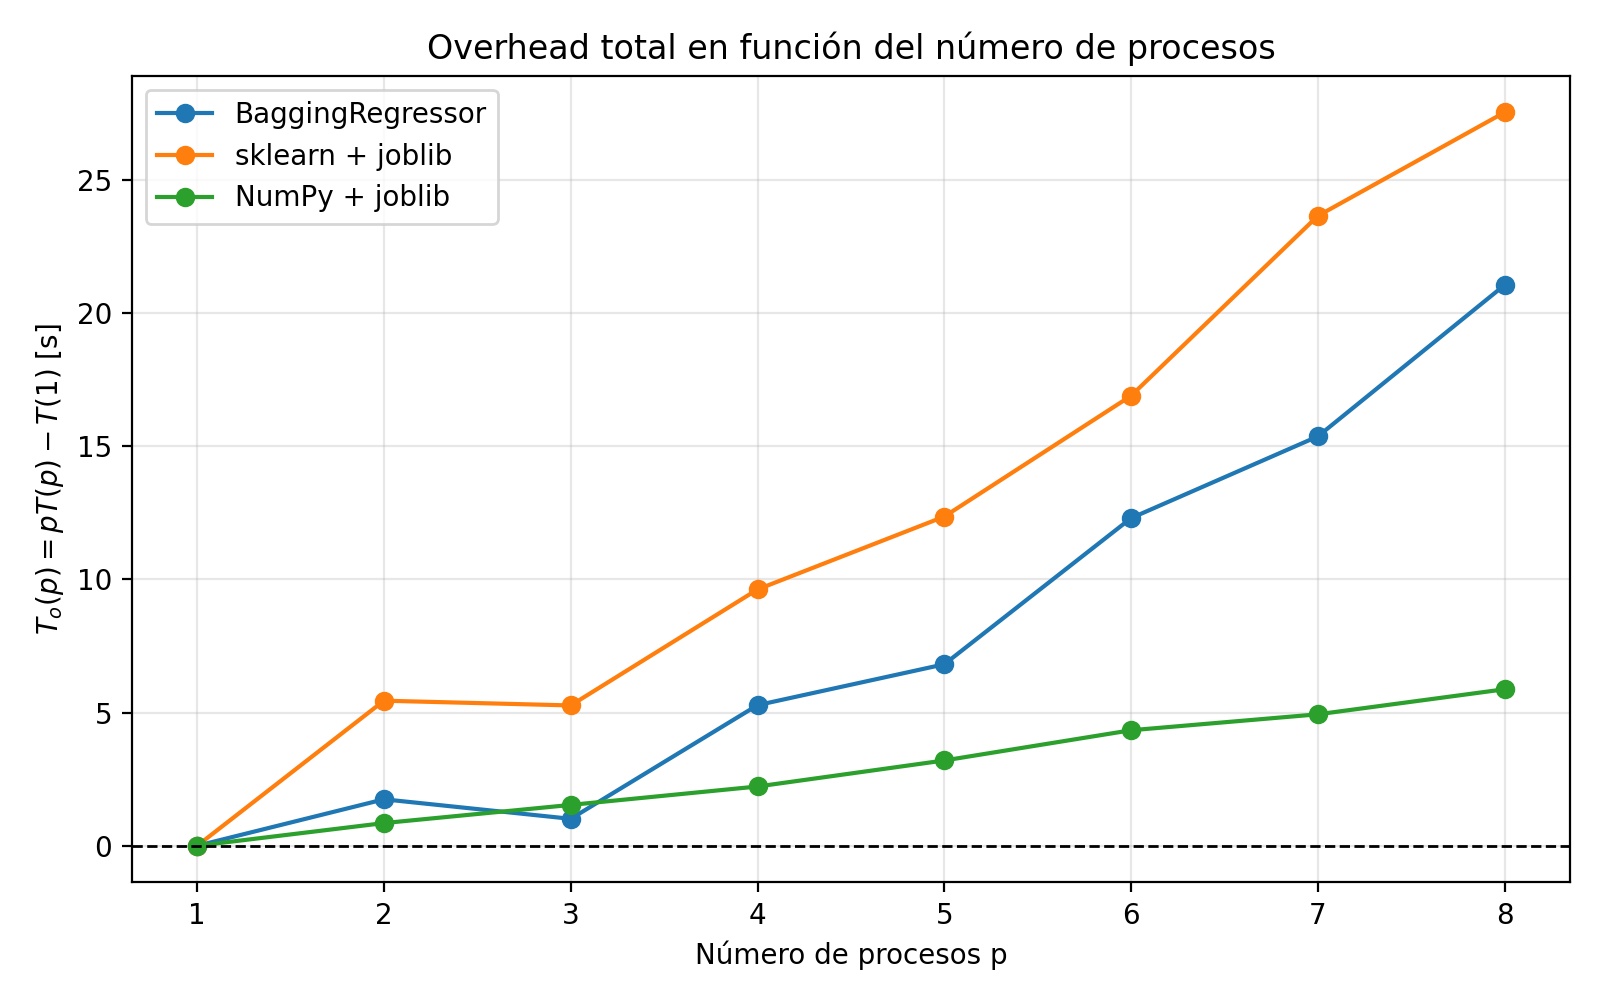
\includegraphics[width=0.82\textwidth]{../results/computer_1/overhead_h.png}
    \caption{Overhead total en función del número de procesos.}
    \label{fig:overhead-h}
\end{figure}

El overhead crece en general con $p$ y explica la separación respecto de la
curva ideal. Sus fuentes principales son el arranque de intérpretes, la
serialización o mapeo de $X$ e $y$, el despacho de las 48 tareas, la creación
de $X^{(b)}$ e $y^{(b)}$, la recolección de coeficientes, la sincronización y
la competencia por memoria y caché. En NumPy el overhead absoluto es menor,
pero es grande respecto de su $T(1)$; por eso no obtiene speedup. Las pequeñas
irregularidades, como el descenso entre $p=2$ y $p=3$ en
\texttt{BaggingRegressor}, corresponden a variabilidad experimental.

\section*{(i) Variación de procesos y threads internos}

Usamos la versión NumPy, que fue la más rápida en (b) y (f), y evaluamos las
20 combinaciones enteras $(p,t)$ que satisfacen $p\,t\leq8$. El límite se aplicó
dentro de cada tarea mediante \texttt{threadpool\_limits(limits=t)}. Cada
combinación se ejecutó cinco veces en un intérprete nuevo y se reportó la
mediana.

\begin{figure}[h]
    \centering
    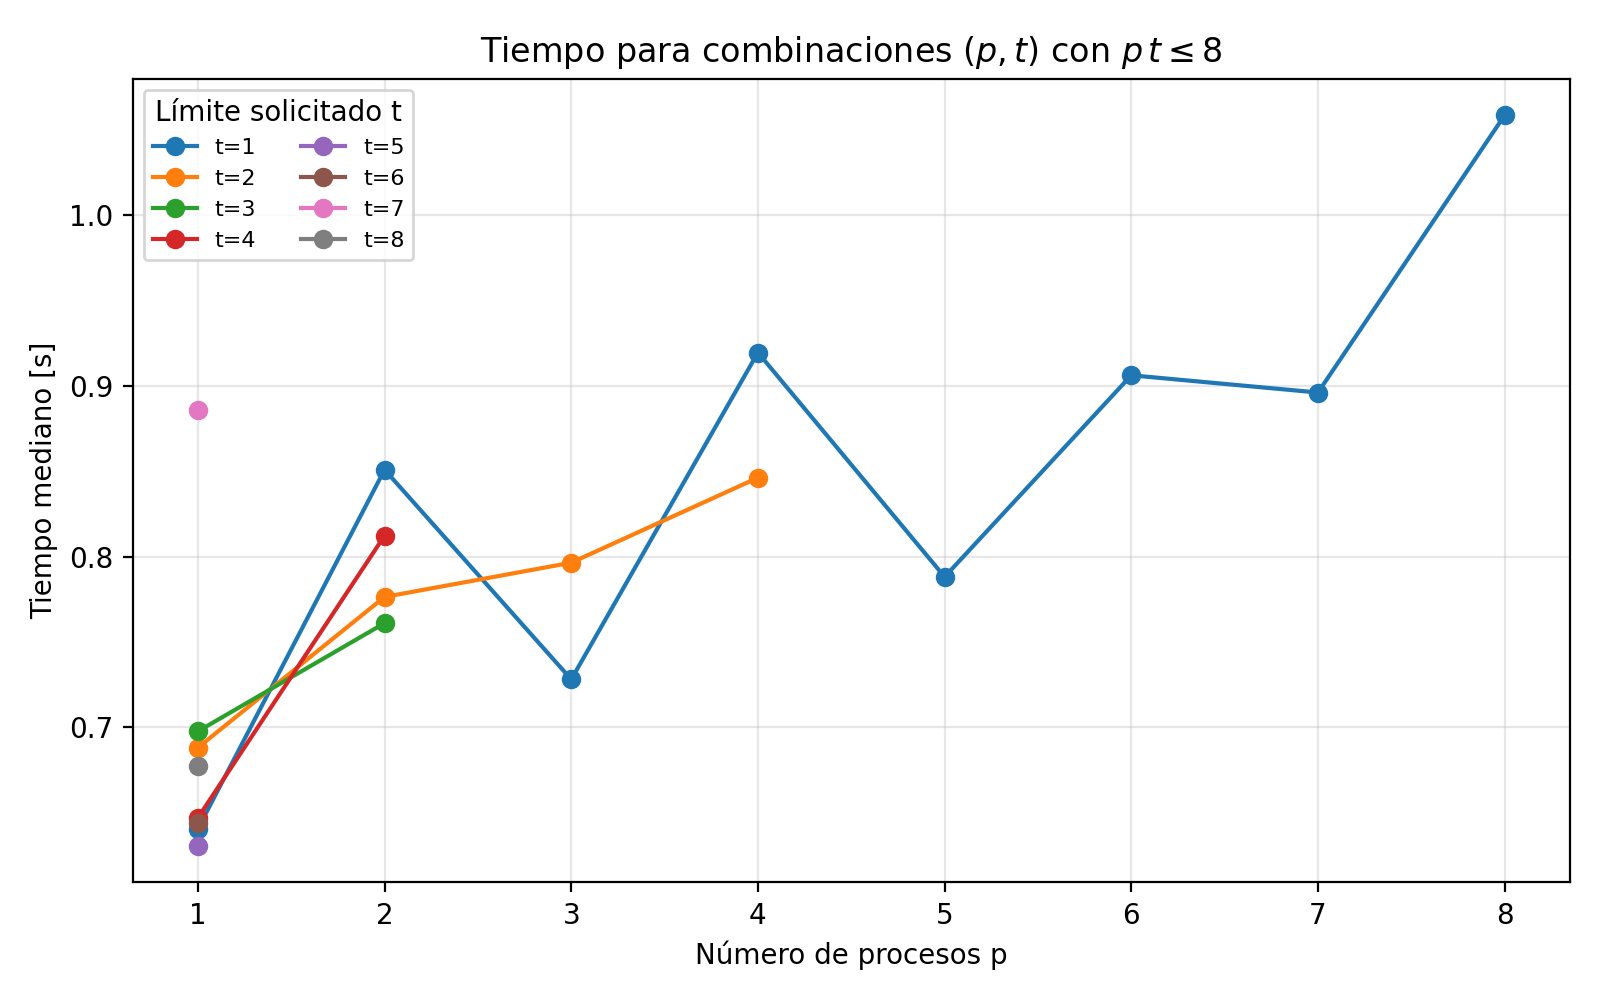
\includegraphics[width=0.82\textwidth]{../results/computer_1/tiempos_i.png}
    \caption{Tiempo mediano para todas las combinaciones $(p,t)$ con
    $p\,t\leq8$.}
    \label{fig:tiempos-i}
\end{figure}

La menor mediana observada fue 0.630 s con $(p,t)=(1,5)$, seguida por 0.640 s
con $(1,1)$, 0.644 s con $(1,6)$ y 0.647 s con $(1,4)$. La diferencia entre
estas configuraciones es pequeña frente a la dispersión de las repeticiones.
Todas las configuraciones con más de un proceso fueron más lentas; por ejemplo,
$(2,3)$ tardó 0.761 s, $(4,2)$ 0.846 s y $(8,1)$ 1.059 s.

Existe una limitación importante: \texttt{threadpool\_info()} no detecta Apple
Accelerate, por lo que $t$ es el límite solicitado, pero no fue posible verificar
el número efectivo de threads internos. En consecuencia, la mejor combinación
nominal es $(1,5)$, pero no hay evidencia suficiente para atribuir su pequeña
ventaja al uso real de cinco threads. La recomendación conservadora para este
problema es $(p,t)=(1,1)$: logra un tiempo estadísticamente comparable, evita
oversubscription y usa menos recursos. Los 100 tiempos individuales están en
\texttt{results/computer\_1/timings\_i.csv}.

\section*{(j) Comparación entre computadores}

Este inciso requiere repetir los experimentos en un segundo computador. Los
scripts aceptan \texttt{--output-dir results/computer\_2} para conservar sus
resultados separados. La comparación final debe informar CPU, cores lógicos,
RAM, sistema operativo, versiones de Python y NumPy, backend BLAS, tiempos,
speedup, eficiencia y mejor combinación $(p,t)$ de ambos equipos. Esta sección
queda pendiente hasta disponer de mediciones reales del segundo computador; no
es correcto extrapolarlas desde el primero.


\section*{Declaración de uso de Inteligencia Artificial}
Se utilizó OpenAI Codex como apoyo para revisar y optimizar el código, diseñar
los experimentos y redactar el informe. Los integrantes del grupo revisaron el
código y validaron experimentalmente los resultados presentados.

\end{document}
